\documentclass{article}

% if you need to pass options to natbib, use, e.g.:
%     \PassOptionsToPackage{numbers, compress}{natbib}
% before loading neurips_2021

% ready for submission
\usepackage{neurips_2021}

% to compile a preprint version, e.g., for submission to arXiv, add add the
% [preprint] option:
%     \usepackage[preprint]{neurips_2021}

% to compile a camera-ready version, add the [final] option, e.g.:
%     \usepackage[final]{neurips_2021}

% to avoid loading the natbib package, add option nonatbib:
%    \usepackage[nonatbib]{neurips_2021}

\usepackage[utf8]{inputenc} % allow utf-8 input
\usepackage[T1]{fontenc}    % use 8-bit T1 fonts
\usepackage{hyperref}       % hyperlinks
\usepackage{url}            % simple URL typesetting
\usepackage{booktabs}       % professional-quality tables
\usepackage{amsfonts}       % blackboard math symbols
\usepackage{nicefrac}       % compact symbols for 1/2, etc.
\usepackage{microtype}      % microtypography
\usepackage{xcolor}         % colors
\usepackage{amssymb}        % símbols de l'AMS
\usepackage{amsmath}        % macros de l'AMS
\usepackage{amsthm, bm}
\usepackage{bigstrut, multicol, multirow, xcolor, rotating}
\usepackage{listings}

% Mathematics definitions and propositions

\newtheorem{theorem}{Theorem}[section]
\newtheorem{propo}[theorem]{Proposition}
\newtheorem{definition}[theorem]{Definition}
\theoremstyle{definition}
\newtheorem{observation}[theorem]{Observation}
\theoremstyle{definition}
\newtheorem{exemple}[theorem]{Example}
\theoremstyle{remark}
\newtheorem*{remark}{Remark}
\newtheorem{comment}[theorem]{Comment}

\makeatletter  
\def\@endtheorem{\qed\endtrivlist\@endpefalse } % insert `\qed` macro
\makeatother
\newtheoremstyle{mythmstyle}{}{}{}{}{\scshape}{.}{ }{}
\theoremstyle{mythmstyle} 
\newtheorem{mythm}{Example}

\newcommand{\Xt}{\textbf{X}_{t|t}}
\newcommand{\Xtt}{\textbf{X}_{t-1|t-1}}
\newcommand{\X}{\hat{\textbf{X}}_{t}}

\title{Kalman Filter for Data Assimilation}

% The following authors' information is not the one displayed. The ones displayed are those written in the .sty

\author{%
  Gerard Castro Castillo\thanks{Thanks to Oriol Pujol for the opportunity.} \\
  Department of Mathematics and Computer Science\\
  University of Barcelona\\
  Barcelona, 08009 \\
  \texttt{gerardc98@gmail.com} \\
  % examples of more authors
  \And
  Flàvia Ferrús\thanks{Thanks to Oriol Pujol for the opportunity.} \\
  Department of Mathematics and Computer Science\\
  University of Barcelona\\
  Barcelona, 08009 \\
  \texttt{flaviaferrus@gmail.com} \\
  % Coauthor \\
  % Affiliation \\
  % Address \\
  % \texttt{email} \\
  % \AND
  % Coauthor \\
  % Affiliation \\
  % Address \\
  % \texttt{email} \\
  % \And
  % Coauthor \\
  % Affiliation \\
  % Address \\
  % \texttt{email} \\
  % \And
  % Coauthor \\
  % Affiliation \\
  % Address \\
  % \texttt{email} \\
}

\begin{document}

\maketitle

\begin{abstract}
  Data assimilation (DA) encompasses a group of statistical methods to improve accuracy of numerical simulation using experimental values. 
  In this paper, DA is leveraged to improve CFD predictions using an optimal method: the Kalman Filter (KF). First, the necessary framework is provided; then, a review of related work is carried out and, finally, then the KF is implemented in R and applied to a turbulent flow use-case. The experimental data is obtained using the flow generated using a fan throughout a cylindrical pipe; while the simulated data obtaining the \texttt{COMSOL} CFD module. 
  The results confirm the benefits of the KF algorithm as means of DA, in view of the huge improvement of the filtered time series in comparison to the raw CFD-simulated one, in terms of bias, variance and correlation with respect to the observations.

  \textbf{Abbreviations:} Data Assimilation - DA, State Space Models - SSM, Kalman Filter - KF, Computational Fluid Dynamics - CFD.
\end{abstract}

\section{Introduction}

The purpose of DA is to determine the best possible forecast state using new real-time \textbf{observations} and short-range \textbf{predictions}. Intuitively, an initial forecast is modelled using the governing equations of the physics system. With this initial distribution, the next-step variable is predicted along with its corresponding covariance matrix (to estimate the forecast error). The groundbreaking idea of the DA approach is an \textbf{additional update step} that uses new real world \textbf{observations} on an experimental system, to improve the predicted values and obtain an analysed state that approximates more accurately the distribution of the real variable, called the \textbf{true state}. The improved predicted state is used on the \textbf{subsequent} time step with new real-time observations.

In order to understand the Kalman recursion we may first need to have a general idea on how to treat time series. We address this in terms of SSM in the following subsection. 
 
\subsection{State space models}

By definition, a \textit{time series} is a set of observations $Y_t$, each one being recorded at specific time $t$, conceived as a random variable that depends on time. In this particular research, we apply the theory for \textit{discrete time series} since the observations are made at fixed-time intervals.
% Generally, the expression of the distribution of a time series is given by a recursive equation, in which we express the dependency of the time series at step $t+1$ in terms of the past steps, and some random noises, $\{X_t_t\}_{t\in T}$. However, this is not the only way to express the distribution of a time series. 
The \textbf{\textit{state-space representation}} arises as an alternative formulation to describe a system's dynamics using two equations. 
% \begin{itemize}
%     \item The \textit{observation equation}, which expresses the $n$-dimensional observation vector $Y_t$ as a linear function of a $k$-dimensional state variable vector, $X_t$, plus noise 
%     \item The \textit{state equation} the state equation, which expresses the $k$-dimensional state vector's $X_{t+1}$ in terms of the previous state $X_t$ and a noise term  
% \end{itemize}
 
\begin{definition}
A time series $\{Y_t\}$ has a state-space representation if there exists a SSM for $\{Y_t\}$, that consists of the observation equation \ref{eq:obs_eq} and the state equation \ref{eq:state_eq} given by:
\begin{align}
    \textbf{Y}_t &= M_t \textbf{X}_t + \textbf{W}_t, \label{eq:obs_eq}
    \\
    \textbf{X}_{t+1} &= F_t \textbf{X}_t + \textbf{V}_t, \label{eq:state_eq}
\end{align}
for $t \in \{0, 1, 2, \dots\}$,  where: $X_t$ is the $k$-dimensional \textbf{state variable vector} of the $n$-dimensional \textbf{observation vector} $Y_t$ ($k\leq n$); $\{\textbf{W}_t\}$, $\{\textbf{V}_t\}$ are distributed as a white noise with $0$ mean and $\{\textbf{R}_t\}$, $\{\textbf{Q}_t\}$ their \textbf{covariance matrices}; $\{ M_t\}$ is a sequence of $(n \times k)$ matrices called \textbf{observation matrices}; and $\{F_t\}$ is a sequence of $(k \times k)$ matrices called \textbf{prediction matrices}. Note that $\{ M_t\}$ and $\{F_t\}$ are \textbf{chosen} as suitable SSM to describe the system.
\end{definition}

\subsection{ARIMA process} \label{arima}

The representation on the SSM is given by the time series distribution of the observations $\bm{Y}_t$. In our study we focus on ARIMA adjusted models, \textit{i.e.} we consider our $\bm{Y}_t$ can be modeled through a certain ARIMA process. The ARIMA(p,s,q) process corresponds to Autorregressive Integrated Moving Average process, with degrees $p,s,q$. The general expression of an ARMA(p,q) time series process, $Y_t$ is given by the Autorregressive part, which indicates the dependency on the previous terms, and the Moving Average part, indicating the modification added by a time dependent white noise $\{X_t\}_{t \geq 0} \sim WN(0, \sigma^2)$. Formally,
$$
Y_t = \sum_{i=1}^p \phi_i Y_{t-i} + X_t + \sum_{i=1}^q \theta_i X_{t-i}, 
$$
The integrated part stands for the times we compute $\Delta Y_t = Y_t - Y_{t-1}$ on the previous time series. More formally, considering the backshift operator $\mathbf{B} Y_t = Y_{t-1}$, then $\{Z_t\}$ is an ARIMA(p,s,q) process if $Y_t := (1-\mathbf{B})^s Z_t$ is an ARMA(p,q) model as described above. 

Naively determining the ARIMA hyper-parameters, \textit{i.e.} $p, s, q$; is generally a bad idea. Instead, to determine the suitable ARIMA distribution of a time series, normality tests are conducted, as well as the autocorrelation and partial correlation analysis. Once an intuitive idea of the time series behaviour is obtained, different ARIMA are models are adjusted to the time series and contrasted by considering the maximum likelihood and lower AIC (Akaike Information Criterion) criterion. Other information criterion can be used (\textit{e.g.} BIC, ...) and there are several libraries which reproduces and optimizes the aforementioned process, such as \texttt{auto.arima} in R, \cite{autoarima} (\textit{Flavia}).

\subsubsection{MA(2): classical expression}\label{ma2}

Let us, for instance, consider an $\texttt{ARIMA}(0,0,2)$ process (or simply $MA(2)$). If $\bm{Y}_t$ has mean $0$, this can be expressed as:
\begin{equation}\label{eq:ma_2}
Y_t = X_t + \theta_1 X_{t-1} + \theta_2 X_{t-2}, \quad \{X_t\}_{t \geq 0} \sim WN(0, \sigma_t^2)    
\end{equation}

The hyper-parameters, in this case $\theta_1, \theta_2$ are statistically estimated. Generally, the corresponding estimates are generally found by applying either the Least Squares method or the Maximum Likelihood method.

\subsubsection{MA(2): SSM representation}\label{ma2_ssm}

Once known the time series fitted distribution $(\theta_1^*, \theta_2^*)$, we can find a SSM formulation. There are many possible representations for an ARIMA process, however following this example of a MA(2), an intuitive and possible SSM representation is given by the following following observation equation \ref{eq:prop_obs} and state equation \ref{eq:prop_state}:
\begin{equation}\label{eq:prop_obs}
     Y_t = ( 1, 0, 0 ) \begin{pmatrix}
    X_{t} \\ X_{t-1} \\ X_{t-2}
    \end{pmatrix} + (0) =: M \mathbf{X}_t + W   
 \end{equation} \begin{equation}\label{eq:prop_state}
     \bm{X}_{t+1} := \begin{pmatrix}
     X_{t+1} \\ X_{t} \\ X_{t-1}
     \end{pmatrix} = \begin{pmatrix}
      0 & 1 & 0 \\ 0 & 0  & 1 \\ 0 & 0 & 0 
     \end{pmatrix}
     \begin{pmatrix}
     X_{t} \\ X_{t-1} \\ X_{t-2}
     \end{pmatrix} + V = F \mathbf{X}_t + V
 \end{equation}
Being $W$ conceivable as white noise with mean 0 and covariance matrix $\mathbf{0}_{3}$; and $V$ distributed as white noise with mean 0 and a covariance matrix $Q$, which should be given in terms of $\theta_1^*, \theta_2^*$. For instance, as seen later in \ref{results}, the \texttt{dlmModARMA} routine of the \texttt{dlm} library, proposes the same SSM representation with:
\begin{equation}
    Q := \begin{pmatrix}
         1 & \theta_1^* & \theta_2^* \\
      \theta_1^* & {\theta_1^*}^2 & \theta_1^* \theta_2^* \\ 
      \theta_2^* & \theta_1^* \theta_2^* & {\theta_2^*}^2
     \end{pmatrix}
\end{equation}

\subsection{Kalman filter}

Given the SSM (not necessarily unique for a system), there is only one optimal estimate of $X_t$ given $\{\textbf{Y}_t\}$ and to find it we will use the KF approach. This KF recursive process consists of two steps at every time point: a \textbf{forecast step}, providing the standard best linear predictor of the state vector, $\hat{\textbf{X}}_t:=P_{t-1}(\bm{X}_t)$; and an \textbf{update step}, which consists on computing the desired analysed estimate, $\textbf{X}_{t|t}:=P_{t}(\bm{X}_t)$ to incorporate the new observations.These two KF steps are described by the following theorems \ref{teor:forecast} and \ref{teor:update}. 
\begin{theorem}[Kalman Filter: forecast step]\label{teor:forecast}
For the state-space model given by the equations \eqref{eq:obs_eq} and \eqref{eq:state_eq}, the one-step predictors $\hat{\textbf{X}}_t:=P_{t-1}(\textbf{X}_t)$ and their error covariance matrices $\Sigma_t = E\left[ (\textbf{X}_t - \hat{\textbf{X}_t})(\textbf{X}_t - \hat{\textbf{X}_t})^T \right]$ are uniquely determined by the initial conditions
\begin{align*}
    \hat{\textbf{X}_1} = P_0(\textbf{X}_1|\textbf{Y}_0), \quad \quad \Sigma_1 = E\left[ (\textbf{X}_1 - \hat{\textbf{X}_1})(\textbf{X}_1 - \hat{\textbf{X}_1})^T \right],
\end{align*}
and the recursions for $t\in \mathbb{N}^{+} \setminus \{1\}$, 
\begin{align}
    \widehat{\textbf{X}}_{t} &= F_{t-1} \widehat{\textbf{X}_{t-1}} + F_{t-1} K(\textbf{Y}_{t-1} - M_{t-1} \widehat{\textbf{X}_{t-1}}),\\
    \Sigma_{t} &= F_{t-1} (I-K M_{t-1})  \Sigma_{t-1}F_{t-1}^T+ Q_{t-1}, \label{KP2} \\
    K&= \Sigma_{t-1} M_{t-1}^T(M_{t-1}\Sigma_{t-1} M_{t-1}^T+ R_{t-1})^{-1},
\end{align}
\end{theorem}

Note the SSM observation equation \ref{eq:obs_eq} and the external data $\textbf{Y}_t$ have not been used yet, but it is on the \textbf{update step} when, according to \ref{teor:update}, the forecast distribution $\widehat{\textbf{X}_t}$ is modified using this new data.

\begin{theorem}[Kalman Filter: update step]\label{teor:update}
The updated estimates $\textbf{X}_{t|t} = P_t(\textbf{X}_t)$ and their covariance matrices $\Sigma_{t|t}= E\left[ (\textbf{X}_t - \textbf{X}_{t|t})(\textbf{X}_t - \textbf{X}_{t|t})^T \right] $ are determined by:
\begin{align}
    \textbf{X}_{t|t}&=\hat{\textbf{X}}_t + K (\textbf{Y}_t - M_t \hat{\textbf{X}_t}), \label{KFteo1}\\
   \Sigma_{t|t}&= \Sigma_t - K M_t \Sigma_t^T,  \label{KFteo2}\\
   K&= \Sigma_t M_t^T(M_t\Sigma_t M_t^T+ R_t)^{-1}.
\end{align}
\end{theorem}

Notice these recursions are remarkably useful in practice. Given the true state variable distribution $X_t$ for a given time $t$ (\textit{e.g.} obtained from numerical computations with CFD), as well as available observations $\{\bm{Y}_1, \dots, \bm{Y}_t\}$, it is possible to obtain a better description $\textbf{X}_{t|t}$ with estimated error (given by the covariance matrix $\Sigma_{t|t}$). In particular, this improved estimation $\textbf{X}_{t|t}$ serves in turn as input for further modeling for the next time step $t + 1$.  
To illustrate this recursive process, the KF algorithm is represented in Figure \ref{fig:diagram}.

\begin{figure}[!ht]
  \centering
  \fbox{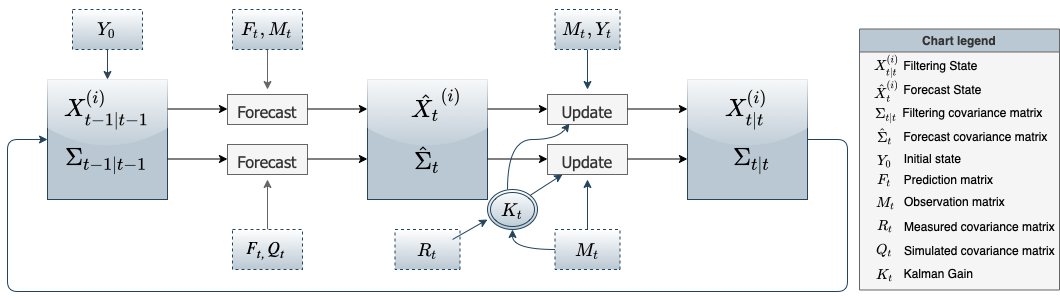
\includegraphics[width=1\textwidth]{img/KF_scheme.png}}
  \caption{(KF information flow chart diagram. Here $i\in \{1, \dots, N\}$, where $N$ either corresponds to the sample dimension in the KF algorithm.}
  \label{fig:diagram}
\end{figure}

% \subsubsection{Ensemble Kalman Filter}\label{EnKF}

% Obtaining a better estimate $\textbf{X}_{t|t}$ gets more complex when we do not have the true state distribution $\textbf{X}$ (\textit{e.g.} when studying not analytical solutions of the \textit{Navier-Stokes} equations). To circumvent this, the Ensemble Kalman Filter (EnKF) arises. In contrast to the standard KF, which works with the entire distribution $\textbf{X}_t$ explicitly, the EnKF forecasts and updates an \textbf{ensemble} of the vectors that \textbf{approximate} the state distribution.
% This sample or ensemble from the distribution results, in turn, in a reduction of the initial dimension of the data set. 

% Specifically, assume that the ensemble $\{ \textbf{X}_{t-1|t-1}^{(1)}, \dots,$ $ \textbf{X}_{t-1|t-1}^{(N)}\}$ is a sample from the updated distribution at time $t-1$. This \textbf{ensemble} is \textbf{forecasted} forward through time and \textbf{updated} when new data become available through the forecast and the update steps; obtaining the ensemble mean: $\overline{\X}$ as the best predictor and $\overline{\Xt}$ as the best estimate. Thus, in the EnKF approach we define the ensemble covariance matrices around the ensemble mean:
% \begin{align*}
%     \Sigma_t^e &= \overline{(\X - \overline{\X})(\X - \overline{\X})^T}, \\
%     \Sigma_{t|t}^e &= \overline{(\Xt - \overline{\Xt})(\Xt - \overline{\Xt})^T}.
% \end{align*}
% And the update step \eqref{teor:update} is adapted, as shown in \cite{evensen2009data}, by formally changing: $K \rightarrow K^e$, $\Sigma_t \rightarrow \Sigma^e_t$, $\Sigma_{t|t} \rightarrow \Sigma^e_{t|t}$, $\X \rightarrow \overline{\X}$ and $\Xt \rightarrow \overline{\Xt}$.

\section{Related work}

The KF was originally presented on \cite{kalman1960new} (\textit{Flàvia}), which introduces an equation for time evolution of the error covariance matrix. The EnKF was then introduced by \cite{evensen1994sequential} (\textit{Flàvia}), presenting improved approaches more orientated to solve nonlinear physical systems with larger number of observations. In particular, the EnKF is an approximate filtering method more capable and efficacious when solving high dimensional and nonlinear systems. In contrast to the standard KF, which works with the entire distribution of the state explicitly, the EnKF stores, propagates and updates an ensemble of vectors that approximates the state distribution, \cite{katzfuss2016understanding} (\textit{Gerard}). Hence, in this EnKF case, the best estimator of the distribution is the mean of the filtered ensembles $\overline{\bm{X}}_{t|t}$, analogously for the best estimator of the covariance matrix $\overline{\Sigma}_{t|t}$. 

In our article, applying KF or EnKF would be essentially the same since the CFD simulatations are deterministic and the state vector distribution will be a single value for each timestep (the same as EnKF with $n=1$ ensembles). Again, the benefits of EnKF are seen in high dimensionality problems, in which it can be conceived as a dimensionality reduction technique. Both sequential methods have later been further developed, implemented and examined in a large number of published papers. Recent studies and reviews on the KF and the EnKF are given from a more theoretical point of view in \cite{evensen2009data} (\textit{Flàvia}) and \cite{brockwell2002introduction} (\textit{Flàvia}), providing detailed information on the formulation, interpretation and implementation of the sequential DA method.

\cite{kato2011hybrid} (\textit{Gerard}) used the EnKF to integrate surface pressures of a square cylinder obtained from computation and experiment, evidencing the capability of reproducing flow fields using the DA method, while they could not be replicated by only numerical simulation. % It was confirmed, too, the EnKF is also more powerful, has computational advantages and provides more accurate results than alternative integrated methods, especially around the measurement points.
\cite{mons2016reconstruction} (\textit{Flàvia}), use the EnKF and other ensemble-based variational DA techniques to reconstruct a 2D unsteady flow past a cylinder combined with a compressible Navier-Stokes flow solver over different system's configurations in order to contrast the various sequential methods implemented.
%over different situations such as uniform and unsteady gust reconstruction, or non-uniform and unsteady boundary conditions and initial field reconstruction.
%gust and initial condition reconstruction and non-uniform and unsteady boundary conditions and initial field reconstruction. %Therefore, various reference states, control vectors, whose dimension ranges from $\approx 10^3$ to $\approx 10^5$, and types of observations are considered, for systems at $Re=100$. 
\cite{deng2018recovering} (\textit{Flàvia}), is focused on the recovery of the global flow field from local quantity measurement data by optimizing the RANS model constants using the EnKF-based assimilation method, paying particular attention on the influence of different observational data on the DA performances and determining the optimal model. 
% Based on the aforementioned approaches and motivations, in this research, the KF and the EnKF were applied to a turbulent wind flow experiment in order to filter and compute the best estimates for the physical configuration. 

\section{Proposal}

The proposed methodology is based on those of \cite{deng2018recovering} (\textit{Flàvia}), \cite{kato2011hybrid} (\textit{Gerard}), \cite{mons2016reconstruction} (\textit{Flàvia}). On the one hand, in particular, it is modeled the turbulent flow of a $2D$ cylindrical configuration (or $3D$ but in virtue of cylindrical symmetry can be studied in $2$ without loss of generality).
% and in virtue of the cylindrical symmetry, the model studied is considered to be in 2 dimensions. Therefore, the NS equations along with the continuity equation are given as follows:
% $$
%     \rho \left(\frac{\partial u}{\partial t} + u  \frac{\partial u}{\partial x} + v  \frac{\partial u}{\partial y}\right) = - \frac{\partial p}{\partial x} + \mu \left(  \frac{\partial^2 u}{\partial x^2} +  \frac{\partial^2 u}{\partial y^2} \right)  
%     $$
%     $$
%     \rho \left(\frac{\partial v}{\partial t} + u  \frac{\partial v}{\partial x} + v  \frac{\partial v}{\partial y} \right) = - \frac{\partial p}{\partial y} + \mu \left(  \frac{\partial^2 v}{\partial x^2} +  \frac{\partial^2 v}{\partial y^2} \right),  
%     $$
%     $$
%     \frac{\partial u}{\partial x} + \frac{\partial v}{\partial y} = 0.
% $$
% TOO technical
% Note that theoretically, considering the Poiseuille flow assumptions, providing the more simple solution of the NS equations, the longitudinal profile of the velocity would be exactly described by a constant value, depending on the transversal position, $u(y)$. In this case, the time series model that would fit more accurately the system would be given by a white noise, this is $ \{X_t_t \sim WN(0, \sigma^2)\}$ meaning that each random vector is a centralized Gaussian with variance $\sigma^2$ and uncorrelated from the rest of times. \\
% However, the real model considered presents some deviations form the ideal case, resulting in the not verification of some assumptions and therefore providing further results from the measured distribution when considering a white noise theoretical distribution. 
On the other hand, the approximation of possible SSM to adjust the experimental distributions are based on ARIMA adjusted models, more specifically on a Moving Average (MA) model.

Essentially, the turbulent flow is modeled assuming the deviation from a parallel steady flow (represented theoretically by a white noise) is due to the interference effects created at the entrance region, as aforementioned, in which the wind flow goes past the inlet with a surface smaller than the pipe's cross-sectional area. The volume expansion provides a dilatation of the flow changing the velocity's direction and affecting the velocity profile, causing a dependence on the past, given either by the MA process or by the differentiated time series describing. 

\subsection{Methodology}

First, we define a physical model based on a wind flow in a finite cylindrical pipe, with associated initial and boundary conditions on the spatial domain using the \texttt{COMSOL} CFD \hyperlink{https://www.comsol.com/cfd-module}{module}. The boundary conditions are given by zero velocity at the upper and lower pipe walls, atmospheric pressure at the outlet and a white noise distributed incoming velocity through the inlet (entrance region at the pipe's edge). The equations governing the system are assumed to be the Reynolds-averaged Navier Stokes (RANS). Of course, the real flow profile has some deviations from the so-called Poiseuille solution of the RANS. This is why DA will prove to be necessary.

Yet, on the one hand, the observation vector, $\bm{Y}_t$, is given by the flow velocity measured experimentally at $p=1$ observation point of the wind flow domain. On the other hand, the state vector, $\bm{X}_t$, represents the velocity flow representation and it is assumed to be distributed as a certain ARIMA, whose exact $p, s, q$ hyper-parameters are found such as the ones adjusting the best the CFD-simulated timeseries in that point. Specifically, the \texttt{COMSOL} CFD simulations are launched at a set of $k\gg p=1$ points and, then, the $\bm{X}_t$ distribution is found out using the simulated timeseries interpolated at the $p=1$ experimental point.  
% In order to compute the study the transversal velocity on the cylinder axis was measured by two anemometers simultaneously placed at two central points of the pipe, point $B$ and point $D$. These samples correspond to the observation data used on the implementation $\mathbf{Y}_t = (Y_t^{(B)}, Y_t^{(D)})$. Additionally, a point next to the entrance region, point $A$ is used as a boundary condition imposed on the CFD simulations implemented on COMSOL, in order to get a first estimate of the real velocity profile. The distribution obtained remains far from the real one, since the ideal assumptions used on the simulation do not hold on the experimental setup, however, by forcing the real distribution of the velocity next to the generator as a boundary condition, the distribution obtained falls in the uncertainty interval, as shown in Figure \ref{fig:implem}. \\
% In order to implement the KF algorithms, the simulated distributions estimated by conducting the corresponding tests. Then, we can define the prediction and observation matrices by describing the SSM formulation for those distributions. The simulated and observation error matrices, given by $Q_t, R_t$ are defined by the diagonal matrices where the nonzero value is given by the simulated error (obtained by conducting the uncertainty propagation) and the observation error (given by the experimental error derived by the anemometer precision). \\

Finally, the KF algorithm is implemented using:
\begin{itemize}
    \item The SSM formulation of the assumed ARIMA distribution for $\bm{X}_t$ interpolated at point $p$. Of course, this SSM description yields the necessary matrices: $M_t$, $F_t$, $R_t$ and $Q_t$.
    \item The observation vector $\bm{Y}_t$ at point $p$.
\end{itemize}

% Thus, we will assume velocity profile follows an $ARIMA(0,1,1)$ distribution. This is an \textit{Integrated Moving Average} model and formally we say 
% $$ Y_t \sim \text{ARIMA}(0,1,1)\ \  \text{if}\ Y_t = Y_{t-1} + \epsilon_t + \theta \epsilon_{t-1},$$
% where $\{ X_t_t\} \sim WN(0,\sigma^2)$ is normal noise with $0$ mean and $\sigma^2$ as covariance matrix. One possible representation of the SSM (not unique), thence, is given by the following observation and state equations
% \color{blue}
% $$
%     Y_t = (\theta, 1) \cdot ( X_{t-1}, X_t)^T = M \mathbf{X}_t 
%     $$
% $$
%     X_{t+1} = (X_{t},  X_{t+1})^T = ([0 , 1], [ 0 , 1 ]) (X_{t-1}, X_t)^T + (0,  \epsilon_t)^T= F \mathbf{X}_t + \mathbf{\varepsilon}_t
% $$

% \begin{equation}\label{eq:prop_obs}
%     Y_t = (\theta, 1) \begin{pmatrix}
%    X_{t-1} \\ X_t
%    \end{pmatrix} = M \mathbf{X}_t     
% \end{equation} \begin{equation}\label{eq:prop_state}
%     X_{t+1} = \begin{pmatrix}
%     X_{t} \\ X_{t+1}
%     \end{pmatrix} = \begin{pmatrix}
%     0 & 1 \\ 0 & 1 
%     \end{pmatrix}
%     \begin{pmatrix}
%     X_{t-1} \\ X_t
%     \end{pmatrix} + \begin{pmatrix}
%     0 \\ \epsilon_t
%     \end{pmatrix}= F \mathbf{X}_t + \mathbf{\varepsilon}_t
% \end{equation}

% Which yields the corresponding prediction, $F$, and observation, $M$, matrices (being $\theta$ unknown). Note the matrices are fixed over time since $F$ expresses the evolution over time of the state vector (theoretically invariable over time) and $M$ expresses the equivalency between the observed and the simulated values (constant in time too).

% Finally, since the errors are assumed to be white noises, the covariance error matrices $R_t$ \& $Q_t$ used on the Kalman recursions are given by the diagonal matrices assuming uncorrelation. Specifically, $R_t$ is given by the experimental errors and $Q_t$ obtained through uncertainty propagation. Since those errors are assumed to be the same over time, they are constant quantities too.   

% On the other hand, the covariance matrices of the measured and simulated errors ($\textbf{W}_t, \textbf{V}_t$, respectively) are considered to be constant over time, and \textbf{diagonal} assuming uncorrelation. The exact error magnitude is given by the experimental and simulated data set standard deviation.

%As the initial condition, we will consider a white noise distributed velocity with mean given by the measured values. \\

\section{Experiments and results}\label{results}

The code\footnote{The code can be found at the authors' repository: \hyperlink{https://github.com/gcastro-98/kf-data-assimilation}{https://github.com/gcastro-98/kf-data-assimilation}} was implemented in R, instead of Python, due to the existence of certain packages in this language that highly simplifies several different steps. In particular, the main obtained results are highlighted below: 
\begin{itemize}
    \item The best ARIMA model adjusting the simulated time series was found using the \texttt{auto.arima} library following the AIC optimization process described at \ref{arima}. The MA(2) process was found as the suitable one with $(\texttt{log likelihood}, \texttt{AIC}, \texttt{BIC}) = (400.76, -795.53, -787.16)$. 

    As described at \ref{ma2}, a MA(2) is uniquely determined by the $(\theta_1, \theta_2)$. In our case, to ensure the simulated time series $\bm{\Tilde{Y}}_t$ had mean $0$ and \eqref{eq:ma_2} could be used, the optimal values were found using the simulated 'displaced' time series $\bm{\Tilde{Y}}_t - \Tilde{\mu}$ with $\Tilde{\mu} =1.0566$ being its mean over time. The found values were: $(\theta_1^*, \theta_2^*)=(0.8505, 0.2416)$.
    \item The SSM formulation of the previous MA(2) was obtained using the \texttt{dlmModARMA} routine from the \texttt{dlm} library. The initial distribution assumed for $X_0$ and its covariance matrix $\Sigma_0$ can be generally determined using the data. However, since the convergence and the achieved results were great enough, the default values were left. The author proposes as initial seeds the following ones, \cite{dlm} (\textit{Gerard}):
    \begin{equation}\label{eq:initials_exp}
         X_0 = ( 0, 0, 0)^T, \quad \Sigma_0 = \mathbb{I}_3 \sigma_0     
    \end{equation} with $\sigma_0 = 10^7$. 
    Then, in this experimental case, the best SSM parameters $M_t$, $F_t$, $R_t$ \& $Q_t$ found were constant in time and found with values:
    \begin{equation}
        M_t = ( 1, 0, 0) \ ; R_t = (0) \ ;\ F_t = \begin{pmatrix}
      0 & 1 & 0 \\ 0 & 0  & 1 \\ 0 & 0 & 0 
     \end{pmatrix} \ ;\  Q_t = \begin{pmatrix}
         1 & \theta_1^* & \theta_2^* \\
      \theta_1^* & {\theta_1^*}^2 & \theta_1^* \theta_2^* \\ 
      \theta_2^* & \theta_1^* \theta_2^* & {\theta_2^*}^2
     \end{pmatrix}
    \end{equation} Note this is the same SSM representation than \ref{ma2_ssm}.
    \item Finally, using the former SSM, the KF is implemented as described by the Kalman recursions given by the Theorems \ref{teor:forecast} and \ref{teor:update}. In our case, the \texttt{dlmFilter} routine of the \texttt{dlm} library was leveraged. The filtered distribution was obtained using as the 'displaced' observations $\bm{Y}_t - \mu $, which after trending it again adding $\mu$, is plotted in Figure \ref{fig:implem}.
\end{itemize}

% Using this distribution, the SSM formulation is described by the observation and state equations as follows:
% \begin{equation}\label{eq:prop_obs_exp}
%      Y_t = ( 1, 0, 0) \begin{pmatrix}
%     Y_{t} \\ \theta_1 \varepsilon_t \\ \theta_2 \varepsilon_{t-1}
%     \end{pmatrix} = M \mathbf{X}_t     
%  \end{equation} \begin{equation}\label{eq:prop_state_exp}
%      X_{t+1} = \begin{pmatrix}
%      Y_{t+1} \\ \theta_1 \varepsilon_{t+1} \\ \theta_2 \varepsilon_{t}
%      %X_{t+1} \\ X_{t} \\ X_{t-1}
%      \end{pmatrix} = \begin{pmatrix}
%       0 & 1 & 0 \\ 0 & 0  & 1 \\ 0 & 0 & 0 
%      \end{pmatrix}
%      \begin{pmatrix}
%      Y_{t} \\ \theta_1 \varepsilon_t \\ \theta_2 \varepsilon_{t-1}
%      X_{t} \\ X_{t-1} \\ X_{t-2}
%      \end{pmatrix} + \begin{pmatrix}
%          1 & \theta_1 & \theta_2 \\
%       \theta_1 & \theta_1^2 & \theta_1 \theta_2 \\ 
%       \theta_2 & \theta_1 \theta_2 & \theta_2^2
%      \end{pmatrix}
%      \begin{pmatrix}
%      \epsilon_{t+1} \\ \epsilon_{t} \\ \epsilon_{t-1} 
%      \end{pmatrix}= F \mathbf{X}_t + W_t \mathbf{\varepsilon}_t. 
%  \end{equation}
% Note that, with some work, it can be proven that this representation is equivalent to the one proposed by the equations \ref{eq:prop_obs} and \ref{eq:prop_state}, since, as aforementioned, the SSM formulation is not unique. 

\begin{figure}[!ht]
  \centering
  \fbox{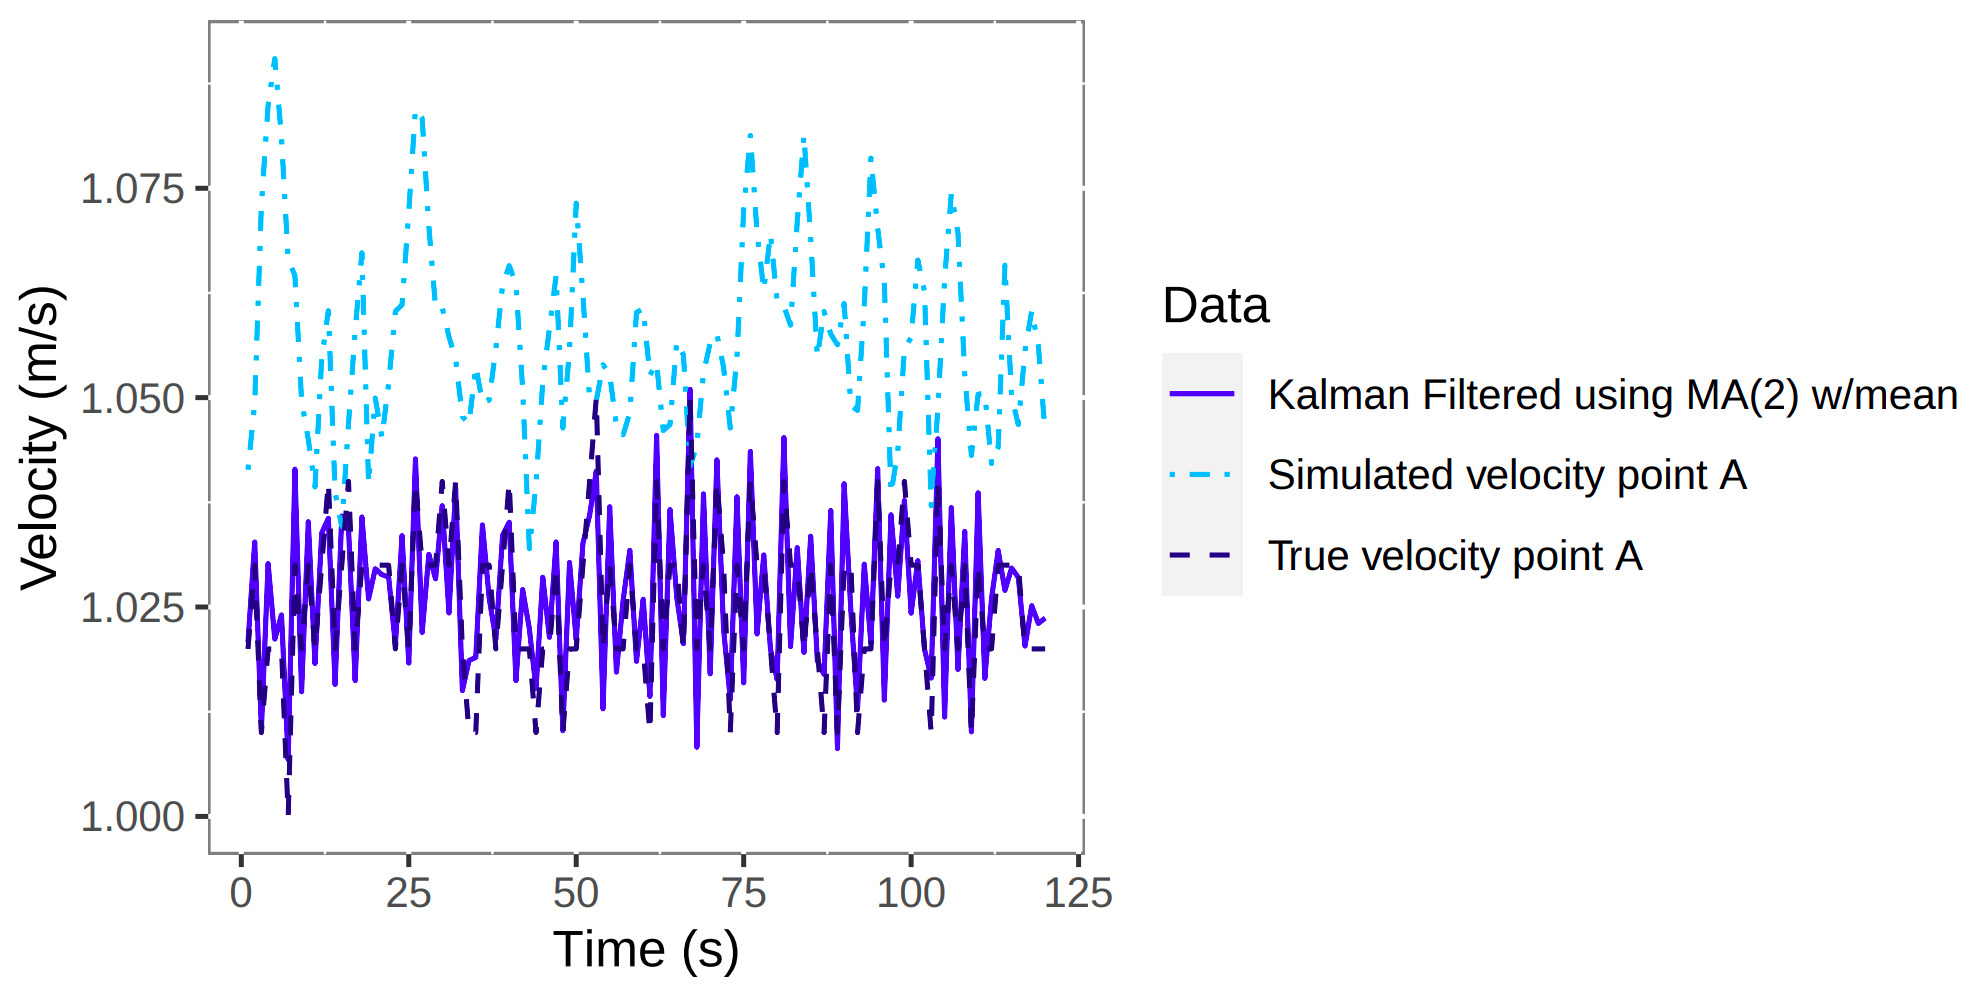
\includegraphics[width=0.8\textwidth]{img/results.png}}
  \caption{Observation (dashed), CFD-simulated (dot-dashed) and KF-filtered (solid) time series of wind flow velocity over time, for an interval of 2 minutes.}
  \label{fig:implem}
\end{figure}

Of course, as it can be appreciated in Figure \ref{fig:implem}, the KF-filtered time series does not adjust completely and perfectly the observations, but does a much better job than the CFD simulation in terms of bias, variance and correlation.

% \subsection{Tables}
% All tables must be centered, neat, clean and legible.  The table number and title always appear before the table. 
% Place one line space before the table title, one line space after the table title, and one line space after the table. The table title must be lower case (except for first word and proper nouns); tables are numbered consecutively.

% \begin{table}
%   \caption{Sample table title}
%   \label{sample-table}
%   \centering
%   \begin{tabular}{lll}
%     \toprule
%     \multicolumn{2}{c}{Part}                   \\
%     \cmidrule(r){1-2}
%     Name     & Description     & Size ($\mu$m) \\
%     \midrule
%     Dendrite & Input terminal  & $\sim$100     \\
%     Axon     & Output terminal & $\sim$10      \\
%     Soma     & Cell body       & up to $10^6$  \\
%     \bottomrule
%   \end{tabular}
% \end{table}

\section{Conclusions}

After this brief and self-contained introduction to the Kalman Filter (KF) algorithm, as well as the presented experimental use-case modeling the wind flow velocity in a finite cylinder, it can be concluded that:
\begin{itemize}
    \item KF constitutes a \textbf{suitable data assimilation strategy} capable of \textbf{highly improving the results} of complex simulations, such as CFD-based ones. 
\end{itemize} 

If the prior distribution of the wind flow profile was known, then KF would not only constitute a suitable way to integrate observations to the predictions, but a powerful tool to model in its own. Powerful but with limitations, nevertheless, because higher lead times (than the very next time step) would yield worse predictions.

Nevertheless, to experience the full potential of the KF algorithm, the KF would have to be implemented iteratively along with the CFD. This is, to apply the filtered states $X_{t|t}$ as the new input for the next time step CFD simulation. 
This would constitute the most natural way to integrate observations and refine CFD simulations. Of course, this would serve as short-term forecast or now-cast model, but other problems would arise: such as the estimation of the suitable distribution for the initial time steps, when not enough simulated data would have been generated...
However, since with the use of warm-up rounds and other advanced strategies may be of use (and which were out of the scope of this work), the authors propose it as a new research line.


%%%%%%%%%%%%%%%%%%%%%%%%%%%%%%%%%%%%%%%%%%%%%%%%%%%%%%%%%%%%

\bibliographystyle{elsarticle-harv}
\bibliography{bibliography}

%%%%%%%%%%%%%%%%%%%%%%%%%%%%%%%%%%%%%%%%%%%%%%%%%%%%%%%%%%%%

\end{document}

\newpage
\appendix

\section{\textbf{Before submission}: check the following things}

\begin{enumerate}

\item For all authors...
\begin{enumerate}
  \item Do the main claims made in the abstract and introduction accurately reflect the paper's contributions and scope?
    \answerTODO{}
  \item Did you describe the limitations of your work?
    \answerTODO{}
  \item Did you discuss any potential negative societal impacts of your work?
    \answerTODO{}
  \item Have you read the ethics review guidelines and ensured that your paper conforms to them?
    \answerTODO{}
\end{enumerate}

\item If you are including theoretical results...
\begin{enumerate}
  \item Did you state the full set of assumptions of all theoretical results?
    \answerTODO{}
	\item Did you include complete proofs of all theoretical results?
    \answerTODO{}
\end{enumerate}

\item If you ran experiments...
\begin{enumerate}
  \item Did you include the code, data, and instructions needed to reproduce the main experimental results (either in the supplemental material or as a URL)?
    \answerTODO{}
  \item Did you specify all the training details (e.g., data splits, hyperparameters, how they were chosen)?
    \answerTODO{}
	\item Did you report error bars (e.g., with respect to the random seed after running experiments multiple times)?
    \answerTODO{}
	\item Did you include the total amount of compute and the type of resources used (e.g., type of GPUs, internal cluster, or cloud provider)?
    \answerTODO{}
\end{enumerate}

\item If you are using existing assets (e.g., code, data, models) or curating/releasing new assets...
\begin{enumerate}
  \item If your work uses existing assets, did you cite the creators?
    \answerTODO{}
  \item Did you mention the license of the assets?
    \answerTODO{}
  \item Did you include any new assets either in the supplemental material or as a URL?
    \answerTODO{}
  \item Did you discuss whether and how consent was obtained from people whose data you're using/curating?
    \answerTODO{}
  \item Did you discuss whether the data you are using/curating contains personally identifiable information or offensive content?
    \answerTODO{}
\end{enumerate}

\item If you used crowdsourcing or conducted research with human subjects...
\begin{enumerate}
  \item Did you include the full text of instructions given to participants and screenshots, if applicable?
    \answerTODO{}
  \item Did you describe any potential participant risks, with links to Institutional Review Board (IRB) approvals, if applicable?
    \answerTODO{}
  \item Did you include the estimated hourly wage paid to participants and the total amount spent on participant compensation?
    \answerTODO{}
\end{enumerate}

\end{enumerate}

\begin{comment}

\section{Paper guidelines}

Formatting instructions: All submissions must be in PDF format. Submissions are \textbf{limited to 6-8 content pages}, including all figures and tables and bibliography.

Evaluation criteria: Submissions will be judged on the basis of their technical quality, novelty, potential impact, and clarity. Typical NeurIPS papers often (but not always) include a mix of algorithmic, theoretical, and experimental results, in varying proportions. While theoretically grounded arguments are encouraged, it is counterproductive to add “decorative math” whose primary purpose is to make the submission look more substantial or even intimidating, without adding significant insight. Algorithmic contributions should have at least an illustration of how the algorithm might eventually materialize into a machine learning application.

\textbf{Expected work: }

Each article is composed of at least 5 sections: \textbf{introduction, related work, proposal, experiments and results, and conclusions}. Bibliography is to be included but does not count on the number of pages for the submission.  You can change the layout and the sections if required by the selected topic or approach. 
Each member of the group must review at least 2 articles on the topic. These are to be included in the background/ state of the art section/ related work section. When the reference is cited please put the name of the member that reviewed that article in brackets. It should look like as follows: `[...] blah blah this cool technique was proposed in [3] (Oriol).' 
The article should focus on the particular problem you selected, you should find and use a dataset showing the problem and on which the solution is to be applied, compare some of the algorithms among them on the selected task, and draw conclusions on that. In this regard, this is like if you were to critizise all the methods, find the limits of application, and benefits.

\end{comment}


\begin{comment}

\textcolor{blue}{Is all what is below necessary after having explained all the former?}

\textcolor{purple}{I don't think it is needed.}

Similarly, the EnKF is implemented in order to contrast results, as described on \cite{katzfuss2016understanding}. The EnKF only requires storing and operating on $N$ vectors (ensemble members) of length $k$ and the calculation of the Kalman gain $K_e$ as described by the ensemble version of the equation of \ref{teor:update} using the sample covariance matrix. \\
As aforementioned, the EnKF algorithm starts with an initial ensemble $\{ \textbf{X}_{0}^{(1)}, \dots,$ $ \textbf{X}_{0}^{(N)}\}$, given by the initial state estimates. Then, at each time step, given the ensemble $\{ \textbf{X}_{t-1|t-1}^{(1)}, \dots,$ $ \textbf{X}_{t-1|t-1}^{(N)}\}$ of draws from the filtering distribution at time $t-1$, the stochastic EnKF\footnote{The EnKF update step could be carried out using deterministic updates, in which the ensemble is approximated by deterministically shifting the prior ensemble, without relying on simulated or perturbed observations.} consists of the two steps implemented over each ensemble's member for $i=1, \dots, N$. Using the corresponding state-space representation of the simulated data, the forecast step involves drawing $\bm{w}_t^{(i)}\sim WN(0, Q_t) $ and calculate $\X^{(i)} = F_t \Xtt^{(i)} + \bm{w}_t^{(i)}$, where the transition matrix has been computed using the time series model that approximates the simulated data, representing the true state distribution. Following up, the update step consists of drawing $\bm{v}_t^{(i)}\sim WN(0, R_t) $ and calculating the filtered state $\Xt^{(i)}= \X^{(i)} + K^e_t (\bm{y}_t + \bm{v}_t^{(i)} - M_t \X^{(i)})$.
\end{comment}